%-------------TO BE COMPLETED-----------------
The planning problem has been studied extensively in various fields like robotics, artificial intelligence, and control theory. In robotics, a classical example of the path planning problem is the \textit{piano-mover's problem}, where the aim is to move a piano from one position to another without colliding with any obstacle. Currently, this problem covers other complications such as non-holonomy, uncertainties, and dynamics.

This chapter covers the preliminaries of path planning and its application on a single agent. The preliminaries are covered in Section.~\ref{sec:prelims}, with topics like \textit{configuration space} and \textit{graph search algorithms}. Then the basic path planning methods are introduced in Section.~\ref{sec:basic_motion_planning}. Section.~\ref{sec:planning_quadrotors} presents the applications of advanced planning methods for quadrotos. Finally, the control methods are shown in Section.~\ref{sec:control_quadrotors}.
\section{Preliminaries}
\label{sec:prelims}
\subsection{Configuration Space}
\label{sec:config_space}
Each distinct situation of a world is called a \textit{state}, $x$, and the set of all possible states is called a \textit{state space}, $X$. The state, $x$, can be transformed to $x'$, by applying an \textit{action}, $u$, as specified by a \textit{state transition function}, $f$, such that:
\begin{align}
	x' = f(x,u)
\end{align}
The set of all possible actions for each state is defined as the \textit{action space}, $U(x)$.

In path planning, we work with a special state space called the \textit{configuration space}, or C-space. The configuration space, $\mathcal{C}$, of a robot is the set of all possible configurations, $x$, that could be achieved by it. The real beauty of C-space is in the way it deals with the obstacles. Suppose that the world, $\mathcal{W}$, contains an obstacle region, $\mathcal{O}$. Assuming that the robot, $\mathcal{A}\subset\mathcal{W}$, the \textit{obstacle region}, $\mathcal{C}_{obs}\subseteq\mathcal{C}$, is defined as
\begin{align}
	\mathcal{C}_{obs} = \{x\in\mathcal{C} | \mathcal{A}(x)\cap\mathcal{O}\neq\emptyset\}
\end{align}
In other words, $\mathcal{C}_{obs}$ is the set of all configurations at which the robot intersects the obstacle region (See Figure.~\ref{fig:conf}). The \textit{free space}, defined as, $\mathcal{C}_{free} = \mathcal{C} \backslash  \mathcal{C}_{obs}$, is the set of all collision free configurations of the robot. 

\begin{figure}
    \centering
    \begin{subfigure}[b]{0.45\textwidth}
        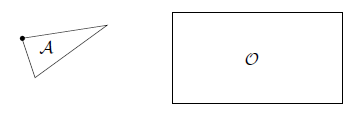
\includegraphics[width=\textwidth]{./images/conf_space_1}
		\caption{The generation of the configuration obstacle $\mathcal{C}_{obs}$}
        \label{fig:conf_1}
    \end{subfigure}
     %add desired spacing between images, e. g. ~, \quad, \qquad, \hfill etc. 
    ~\begin{subfigure}[b]{0.45\textwidth}
        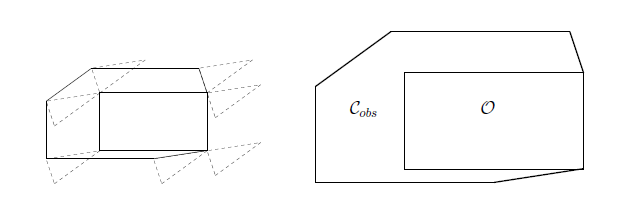
\includegraphics[width=\textwidth]{./images/conf_space_2}
		\caption{The configuration space is obtained by sliding the triangle around the obstacle while keeping them both in contact}
		\label{fig:conf_2}    
	\end{subfigure}
    \caption[Visualization of configuration space obstacle]{Visualization of configuration space obstacle \cite{lavalle2006planning}}
    \label{fig:conf}
\end{figure}


Let $x_I \in \mathcal{C}_{free}$ and $x_G \in \mathcal{C}_{free}$ be the \textit{initial configuration} and  the \textit{final configuration} respectively. A path planning algorithm aims to compute a continuous path starting at $x_I$ and ending at $x_G$. 

\subsection{Graph Search Algorithms}
\label{sec:graph_search_algo}
\textit{State transition graph} is a convenient tool that could be used to approach path planning problems. In the graph $\mathcal{G}$, the states and actions form the vertices $\mathcal{V}$ and directed edges $\mathcal{E}$ respectively. A directed edge  from $x\in X$ to $x'\in X$ exists only if there exists an action $u\in U$ such that $x'=f(x,u)$. With this representation, the graph search algorithms could be directly applied to the path planning problem.

In this section, we cover the major graph search algorithms like breadth first search, length first search and A* search. These forward search algorithms start at the initial state and explores the graph until encountering the goal state. The general template of such algorithms \cite{lavalle2006planning} is shown in Algorithm~\ref{alg:fsearch}.

\begin{algorithm}
\caption{Forward Search}\label{alg:fsearch}
\begin{algorithmic}[1]
%\Procedure{Euclid}{$a,b$}
\State $Q$.Insert($x_I$) and mark $x_I$ as visited
\While{$Q$ not empty}
\State $x\gets Q$.GetFirst()
\If{$x\in X_G$}
\State \textbf{return} SUCCESS
\EndIf
\ForAll{$u\in U(x)$}
\State $x'\gets f(x,u)$
\If{$x'$ not visited}
\State Mark $x'$ as visited
\State $Q$.Insert($x'$)
\Else
\State Resolve duplicate $x'$
\EndIf
\EndFor
\EndWhile
\State \textbf{return} FAILURE
\end{algorithmic}
\end{algorithm}

During the search, there will be three kinds of states. The \textit{unvisited} list consists of all the unexplored states of graph. If a state, along with all its next possible states, have been visited, it is added to the \textit{dead} list. The remaining states, i.e. the explored states with unexplored neighbours, forms the \textit{alive} list. As shown in the Algorithm~\ref{alg:fsearch}, the alive list is stored in a data structure $Q$. The main difference between the search algorithms is in the way they sort $Q$. 

In \textit{breadth first search}, $Q$ is implemented as a First-In-First-Out (FIFO) queue. This results in a uniform expansion of the search frontier. If we make $Q$ a stack, the graph would be explored aggressively in an arbitrary direction, resulting in the \textit{depth first search}. 

If we know the cost of the actions, we could use that to increase the efficiency of the search algorithm. In \textit{Dijkstra's algorithm}, $Q$ is sorted according to the \textit{cost-to-come} function, $C(x)$, which is defined as the minimum cost  of travelling from $x_I$ to $x$ according to the current knowledge. 

In many cases, it is possible to obtain a heuristic estimate of the cost to reach the goal from any state. Let this function be called $\hat{G}(x)$. This knowledge can be exploited to reduce the number of states explored to reach the goal. The \textit{A* search algorithm} sorts $Q$ according to the sum $C(x) + \hat{G}{x}$.


\section{Basic Path Planning Methods}
\label{sec:basic_motion_planning}
As mentioned before, the path planning problems are defined in the configuration space, whereas the graph search algorithms are based on graphs. To connect these problems, we should reformulate the path planning problem, framed on a continuous configuration space, in terms of a graph. This section is dedicated to three different methods of approaching this problem: grid based, potential field based, and sampling based.
\subsection{Grid Based Approach}
\label{sec:grid_search}
In this approach, initially, a grid of locations is sampled in the configuration space. Each vertex $\mathcal{V}$ of the graph represent a configuration. A collision-check function is ran on each grid to check if it is in $\mathcal{C}_{free}$. It is assumed that the grids are close enough in space such that there can be no obstacle between two adjacent grids. In other words, we assume that if two adjacent vertices are in $\mathcal{C}_{free}$, every point in the line joining them is also in the $\mathcal{C}_{free}$. Therefore, we join the vertices by an edge. This discretizes the set of actions, and hence the grid search algorithms can be applied to find the path from the start to the goal. 

Grid based search works well for low dimensional problems. However, this method is computationally infeasible for high-dimensional systems, since the number of points on the grid increase exponentially with configuration space dimension. 

\subsection{Sampling-based Approach}
\label{sec:sampling_search}
Sampling-based search algorithms are the leading methods to tackle higher-dimensional path planning problems. These approaches chooses the points in the configuration space randomly, instead of uniformly, to generate the graph. In other words, the connectivity of $\mathcal{C}_{free}$ is explored by sampling random configurations and trying to connect in a network. Two major sampling-based methods: \textit{rapidly-exploring random trees} (RRT) \cite{lavalle2006planning} and \textit{probabilistic roadmaps} \cite{kavraki1994probabilistic}, are discussed in this section.

\subsubsection{Probabilistic Road-Map (PRM)}
Probabilistic roadmap is the preferred method if the initial and goal states are not fixed. This method consists of two stages: a preprocessing and query stages. The pseudocode of this method is shown in Algorithm.~\ref{alg:prm}.
In the preprocessing stage, a random configuration is generated, and neighbours within a predefined distance are connected if all the points in the line joining them are in $\mathcal{C}_{free}$. This step is repeated until a dense graph is generated (see Figure.~\ref{fig:prm}). 

In the query stage, the start and goal configurations are connected to the graph, and an appropriate search algorithm is used to find the path. Once the roadmap has been constructed, it can be used to generate paths between various start and goal locations, as long as the environment is static. This justifies the initial cost of constructing the graph. 

However, in many cases, we are only interested in planning between one specific start and goal locations, and therefore, building a roadmap for such problems is wasteful. In such situations, it would be better to consider approaches that explicitly uses the initial and goal locations in approaching the problem.


\begin{algorithm}
\caption{Probabilistic Road-Map}\label{alg:prm}
\begin{algorithmic}[1]
\State $\mathcal{G}$.init($i\gets 0;$)
\While{$i<N$ }
\If {$\alpha(i)\in \mathcal{C}_{free}$}
\State $\mathcal{G}$.add\_vertex($\alpha(i)$); $i\gets i+1$
\For \textbf{each} $q\in \text{NEIGHBORHOOD}(\alpha(i),\mathcal{G})$
\If {(\textbf{not} $\mathcal{G}$.same\_component($\alpha(i),q$)) \textbf{and} CONNECT($\alpha(i),q$)}
\State $\mathcal{G}$.add\_edge($\alpha(i),q$)
\EndIf
\EndFor
\EndIf
\EndWhile
\State \textbf{return} $\mathcal{G}$
\end{algorithmic}
\end{algorithm}

\begin{figure}
\centering
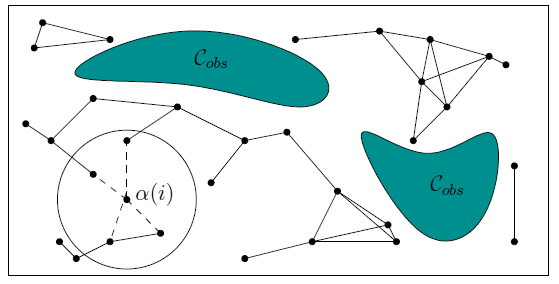
\includegraphics[width=0.6\textwidth]{./images/prm}
\caption[Preprocessing stage of PRM]{Preprocessing stage of PRM. The new randomly sampled point $\alpha(i)$ is connected to the neighbouring vertices in the roadmap}
\label{fig:prm}
\end{figure}


\subsubsection{Rapidly-Exploring Random Trees (RRT)}
The RRT algorithm explores the space by randomly sampling a space-filling \textit{tree}. A tree is a special graph, with every vertex connected to a single parent. As shown in Algorithm~\ref{alg:rrt}, with each new sample $\alpha(i)$, a vertex $q_s$ is added between it and the nearest state $q_n$ in tree. $q_s$ lies at a distance $\delta$ from $q_n$ on the line joining $\alpha(i)$ and $q_n$. If $\alpha(i)$ lies in the obstacle region, $q_s$ is generated at the edge of the obstacle as shown in Figure~\ref{fig:rrt}. 

This algorithm is very efficient in exploring the free space starting from a configuration. In order to use this for our problem, we usually generate two RRTs, one rooted at the initial configuration and the other at the goal configuration. We then grow both trees until they meet. There are many variations of RRT methods, and they are very effective at tackling high dimensional problems. They can also handle problems with kinodynamic constraints.

\begin{algorithm}
\caption{Rapidly-exploring Random Trees}\label{alg:rrt}
\begin{algorithmic}[1]
\State $\mathcal{G}$.init($q_0$)
\For{$i$ = 1 \textbf{to} $k$}
\State $q_{rand}\gets$RAND\_CONFIG()
\State $q_{near}\gets$NEAREST\_VERTEX($q_{rand},\mathcal{G}$)
\State $q_{new}\gets$NEW\_CONF($q_{near}, q_{rand}, \Delta q$)
\State $\mathcal{G}$.add\_vertex($q_{new}$)
\State $\mathcal{G}$.add\_edge($q_{near},q_{new}$)
\EndFor
\State \textbf{return} $\mathcal{G}$
\end{algorithmic}
\end{algorithm}

\begin{figure}
\centering
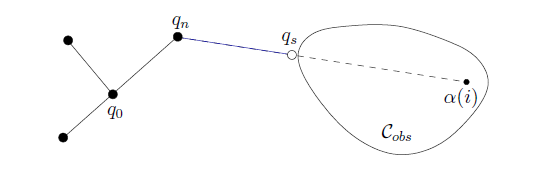
\includegraphics[width=0.6\textwidth]{./images/rrt}
\caption[Tree expansion in RRT]{If the sampled point $\alpha(i)$ lies inside the obstacle region, the new vertex $q_s$ is formed at the boundary of $\mathcal{C}_{obs}$}
\label{fig:rrt}
\end{figure}

The main issue with sampling based approaches is they are not \textit{complete}: i.e. they cannot guarantee the absence of a path even if they are unable to find it. These algorithms are \textit{probabilistically complete}, which means that with enough points, the probability that it finds an existing solution converges to one.
\subsection{Potential field based Search}
\label{sec:pot_search}
Potential field based approaches generate good results with minimal computations. In this method, the robot (represented in C-space), is treated as a particle under the influence of an artificial potential field. The potential field is designed in such a way that the goal has an \textit{attractive potential} and the obstacles has a \textit{repulsive potential}. This ensures that the robot moves towards the goal while avoiding obstacles. 

As shown in Figure.~\ref{fig:potential}, this method can be visualized as a particle moving on a 2D plane under gravity. The goal and the obstacles are represented by a basin and hills respectively. At every instance, the robot tries to move in a direction along decreasing potential, thereby finally reaching the goal. This is done by using the gradient of the potential function to steer the robot. The control velocity \textbf{v} is chosen as:
\begin{align}
\textbf{v} \propto -\nabla f_c
\end{align}

Using this approach, the robot can generate a path by just knowing the potential function. The potential field can be computed by the knowledge of the robot's position, and local sensor data. Moreover, the gradient could be evaluated by using simple finite difference methods. The simplicity of this method makes it appealing to robotic applications. However, this method may find a non-optimal path, or no path at all if the particle is stuck in a local minima.

%\begin{figure}
%\centering
%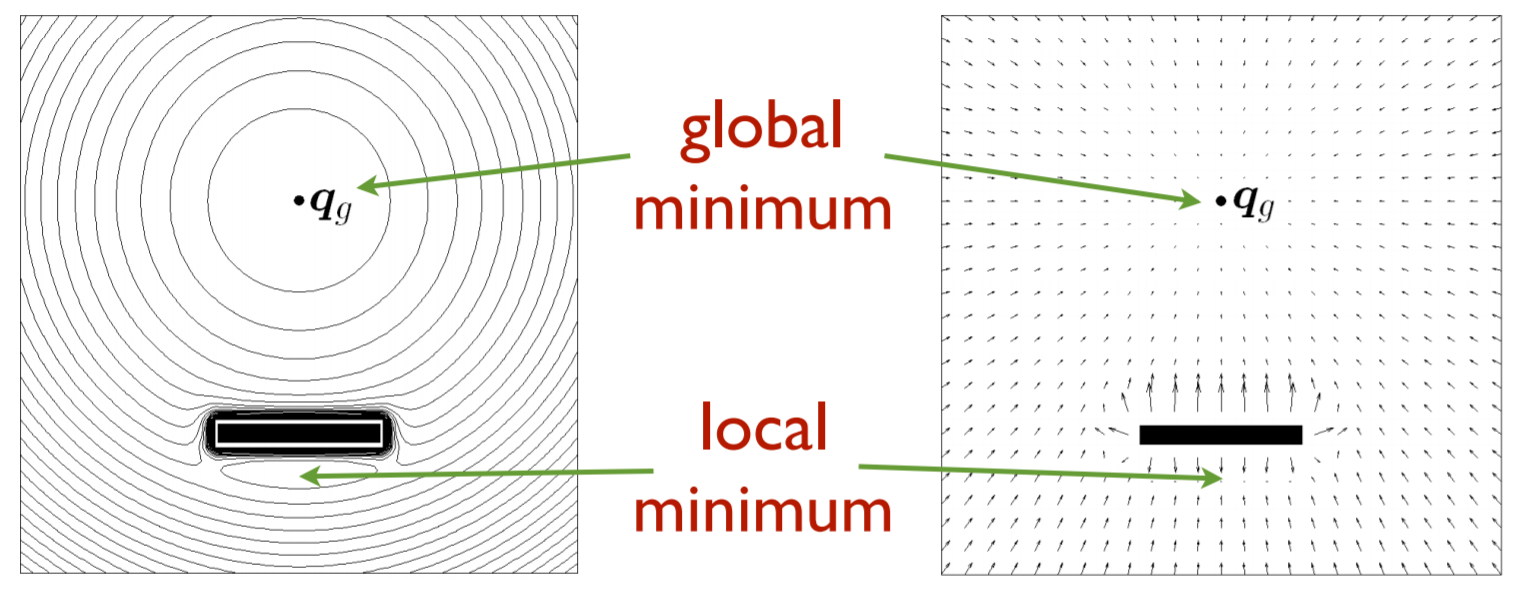
\includegraphics[width=0.6\textwidth]{./images/potential_search}
%\caption[Local minima in potential field based search]{Local minima in potential field based search. \cite{siciliano2010robotics}}
%\label{fig:potential_search}
%\end{figure}

\begin{figure}
    \centering
    \begin{subfigure}[b]{0.3\textwidth}
        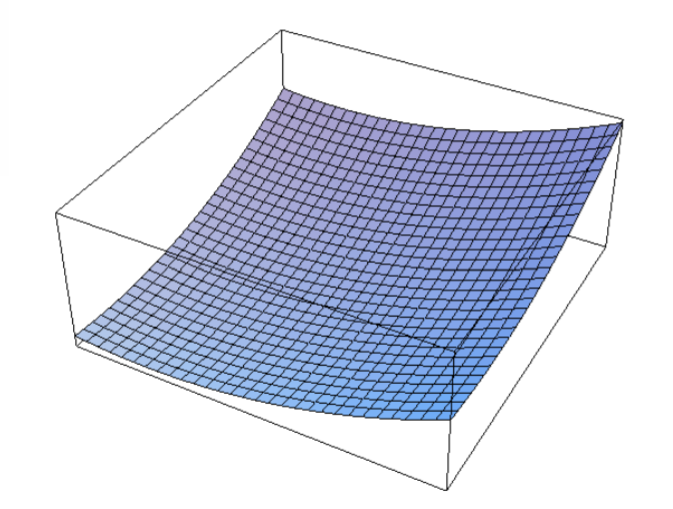
\includegraphics[width=\textwidth]{./images/potential_goal}
		\caption{The goal modelled as an attractive potential field, $f_a$}
        \label{fig:potential_goal}
    \end{subfigure}
     %add desired spacing between images, e. g. ~, \quad, \qquad, \hfill etc. 
    ~\begin{subfigure}[b]{0.3\textwidth}
        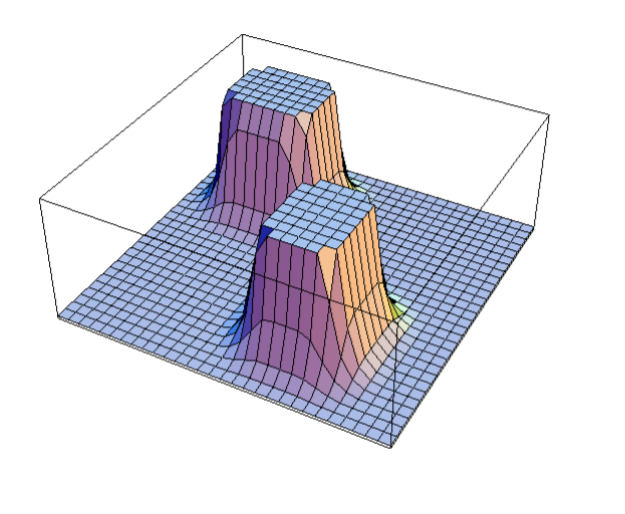
\includegraphics[width=\textwidth]{./images/potential_obs}
		\caption{The obstacles are modelled as a repulsive potential field, $f_r$}
		\label{fig:potential_obs}    
	\end{subfigure}
    ~\begin{subfigure}[b]{0.3\textwidth}
        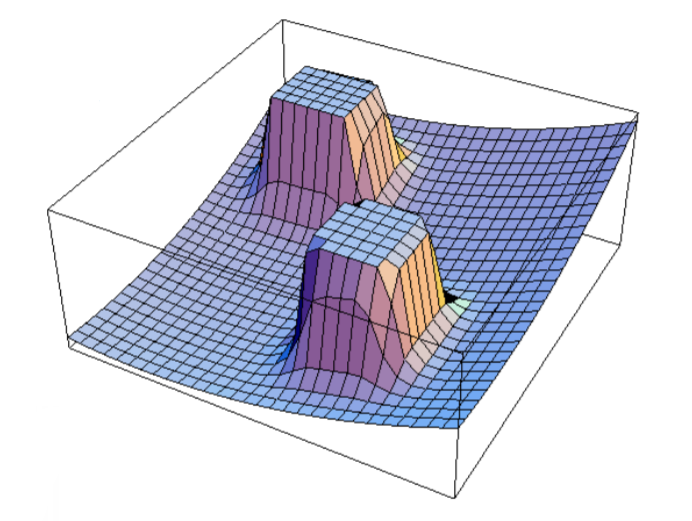
\includegraphics[width=\textwidth]{./images/potential_combined}
		\caption{The combined potential field, $f_c=f_a+f_r$}
		\label{fig:potential_combined}    
	\end{subfigure}	
    \caption[Visualization of potential field based search]{Visualization of potential field based search \cite{lavalle2006planning}}
    \label{fig:potential}
\end{figure}

\section{Kinodynamic Path Planning}
\label{sec:kinodynamic}
Until now, we assumed that the path between any two configurations can be easily determined. However, this might not always be possible in most planning problems in mechanical systems due to the kinematics and dynamics constraints. Planning in such a situation is called \textit{kinodynamic} path planning. 

A classical approach to this problem is to decompose it into two sub-problems. Initially, collision-free a geometric path, called the quasi-static solution, is computed. It can be visualized as a trajectory that the robot can follow in very slow speeds and reach the goal. In the next step, a constrained optimization problem is solved to minimize the time taken to follow the trajectory while respecting the dynamic constraints. 

This decoupled approach is very efficient in finding feasible paths. However, they do not obtain good quality paths since the dynamics is not considered during the path planning stage. To obtain better results, more complex \textit{direct planning} methods are preferred. 

Even though there exists many deterministic approaches like based on optimal control, numerical optimization, and grid search, sampling-based approaches are preferred to solving these problems due to their high dimensionality. In this case, we have to rethink the way in which we connect two configurations. 

The direct way to do is to solve a two-point boundary value problem (BVP). However, this is computationally demanding and hence infeasible for most scenarios. If the dynamics is linear or could be linearized about an operation point, we could use LQR based techniques to obtain faster results. Some researchers bypass the solving of BVP by using precomputed \textit{motion primitives}.

The most studied method is the forward propagation of dynamics. New states are generated by performing a feasible action on states that are already generated, typically by using ODE solvers. This method works well with RRT and has generated good results. 

Now that we have seen the complexities of planning in mechanical systems, we move ahead to studying the path planning problem for quadrotors.

\section{Motion Planning for Quadrotors}
\label{sec:planning_quadrotors}
This section is dedicated to motion planning methodologies for quadrotors. 
Our aim is to develop a planner that generates a feasible path, that respects the input and dynamics constraints, to bring the quadrotor to the goal as soon as possible. To achieve this, we should exploit the internal dynamics of the quadrotor. Furthermore, it should find plans in real-time at rates around 50 Hz. 

In general, there are two approaches to deal with this problem. In the first approach, the problem is solved by dividing it into global and local planning sub-problems. The global planner, typically implemented using sampling based search, computes a set of configurations through which the quadrotor should move to reach the goal while avoiding collisions. Then the local planner generates time parametrized \textit{trajectories} that can be realized by the vehicle. The local planning problem is often called as trajectory generation. 

This method is simpler, but it may not lead to a global optimum as the initial dynamics of the robot is not considered in planning. In the second approach, a global minimum is usually obtained by discretizing the state-space into a finite lattice using precomputed motion primitives. 

The second approach relies on the differential flatness \cite{mellinger2011minimum} property of the quadrotor dynamics to derive constraints on the trajectory and then solves an optimization problem to find the optimum trajectory. Some interesting state-of-the-art path planning methodologies are discussed in this section. 
%--------------QUADROTOR MODELLING (MAYBE)---------------
% Minimum snap

\subsection{Sampling-Based Motion Planning}
\label{sec:sampling_planning}
%Gradient-Based Online Safe Trajectory Generation
%for Quadrotor Flight in Complex Environments
As mentioned before, the high dimensionality of the path planning problem makes it infeasible for simple-graph search based algorithms. Sampling-based methods perform better in this case, especially in cluttered environments. In this section, we briefly introduced some sampling based approaches. 

Some popular sampling based path-planning algorithms include, RRT*, PRM* (Probabilistic Road Map*) and rapidly-exploding random graphs (RRG), which is an extension of RRT. The approach in \cite{webb2013kinodynamic}, the RRT* method is combined with a fixed-final-state-free-final-time controller to obtain asymptotic optimality. Closed-form solutions of optimal trajectories could be derived in this method. 

Bry and Roy et al. \cite{bry2011rapidly} combined the belief roadmap with RRG to address the problem of motion planning in the presence of state uncertainty. The resultant search tree in belief space is provably convergent to the optimal path. Shen et al. \cite{shen2017gradient} used RRG method, along with a trajectory optimization framework, to generate a safe, smooth and dynamically feasible trajectory based on the piecewise line segment initial path. 

\subsection{Polynomial-Based Motion Planning}
\label{sec:poly_based_planning}
A trivial trajectory that passes through a set of \textit{waypoints} is the one that interpolates them using straight lines. Evidently, this trajectory isn't efficient as the robot has to come to rest at each waypoint. In this section, we discuss in detail the work by Kumar et al. \cite{mellinger2011minimum}, which generates a \textit{minimum-snap trajectory} that passes through the waypoints while satisfying the constraints on velocity and accleration. 

In this work, the trajectories are parametrized as piecewise polynomial functions of $n^{th}$ order over $m$ time intervals as:
\begin{align}
  \sigma_{t} =
    \begin{cases}
      \sum_{i=0}^n \sigma_{Ti1}t^i& t_0\leq t\leq t_1\\
      \sum_{i=0}^n \sigma_{Ti2}t^i& t_1\leq t\leq t_2\\
      &\vdots\\
      \sum_{i=0}^n \sigma_{Tim}t^i& t_{m-1}\leq t\leq t_m
    \end{cases} 
\end{align}
The decision variable vector, $\textbf{c}$, is a $3mn\times 1$ vector consisting of the constants $\sigma_{T{ij}}$.The optimization program minimizes the $k_r^{th}$ derivative of the square of the position as:
\begin{align}
\begin{split}
\min_{\textbf{c}} \quad & \int_{t_0}^{t_f} \left\Vert\frac{d^{k_r}\textbf{r}_T}{dt^{k_r}})\right\Vert^2 dt\\
\textrm{s.t.} \quad & \textbf{r}_{T}=\textbf{r}_w, \quad w=0,\ldots,m\\
  &\left.\frac{d^j x_T}{dt^j}\right\rvert_{t=t_w}=0\text{ or free,}w=0,\ldots,m;j=1,\ldots,k_r\\
  &\left.\frac{d^j y_T}{dt^j}\right\rvert_{t=t_w}=0\text{ or free,}w=0,\ldots,m;j=1,\ldots,k_r\\
  &\left.\frac{d^j z_T}{dt^j}\right\rvert_{t=t_w}=0\text{ or free,}w=0,\ldots,m;j=1,\ldots,k_r
\end{split}
\end{align}
Here, $\textbf{r}_T=[x_T,y_T,z_T]^\top$ and $\textbf{r}_i=[x_i,y_i,z_i]^\top$. It is also ensured that the first $k_r$ derivatives of the position is continuous. The optimization problem can be formulated as a quadratic program:
\begin{align}
\begin{split}
\min \quad & \textbf{c}^\top \textbf{H} \textbf{c} + \textbf{f}^\top\textbf{c} \\
\textrm{s.t.} \quad &\textbf{Ac}\leq \textbf{b}
\end{split}
\end{align}

As the inputs to the system was found to be functions of the fourth derivatives of positions, $k_r$ was chosen to be 4, and hence the snap was minimized. This rise to smooth trajectories that avoid paths involving extreme control inputs. Moreover, the resulting smoothness helps in maintaining the quality of onboard sensor measurements. Then, the segment times are optimized to minimize the total time. 

The method presented in  \cite{richter2016polynomial} jointly optimizes polynomial path segments in an unconstrained quadratic program to solve the minimum-snap trajectory problem. The output is numerically stable for high-order polynomials and large numbers of segments. As shown in Figure.~\ref{fig:bry_poly}, they generated fast flight paths through cluttered environments by coupling this technique with an appropriate kinematic planner. In addition, an implicit segment time allocation strategy, based on a single user-defined parameter on aggressiveness, led to far superior results.

\begin{figure}
\centering
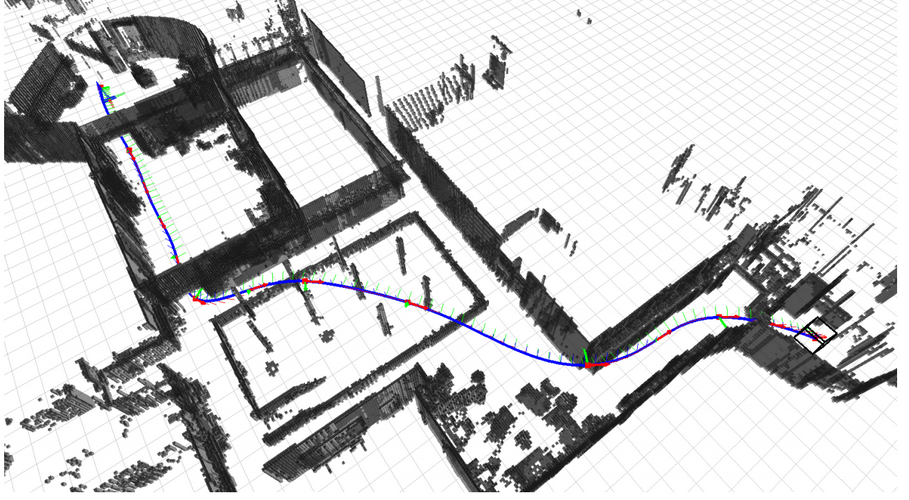
\includegraphics[width=0.6\textwidth]{./images/bry_poly.png}
\caption[Minimum-snap trajectory generation using unconstrained quadratic program]{Minimum-snap trajectory generation using unconstrained quadratic program. \cite{richter2016polynomial}}
\label{fig:bry_poly}
\end{figure}


\subsection{Search-Based Motion Planning}
\label{sec:search_based_planning}
%Search-based Motion Planning for Quadrotors using
%Linear Quadratic Minimum Time Control
Recent work by Kumar et al. \cite{kumar2017search} aims at computing globally optimum, collision-free, minimum-time, dynamically-feasible trajectories in real-time. When the geometric path is first computed and then smoothened, the generated trajectory may not contain a globally optimum trajectory as this approach does not consider the initial dynamics of the robot. As shown in Figure.~\ref{fig:search_kumar}, the trajectory generated by this approach is superior to other approaches. 

\begin{figure}[h!]
\centering
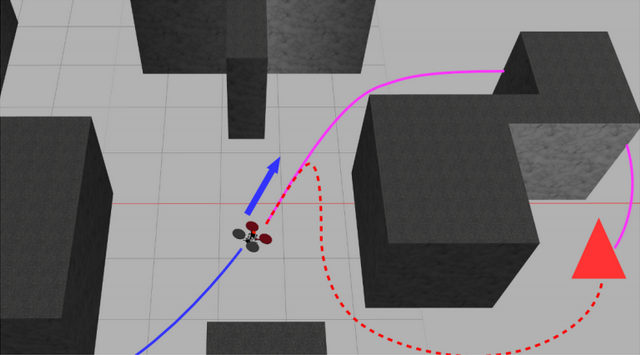
\includegraphics[width=0.6\textwidth]{./images./search_kumar.png}
\caption[Path planning performed at non-zero inital velocity.]{Path planning performed at non-zero inital velocity. The search based approach shown in \cite{kumar2017search} generates the more natural and time optimal magenta curve, where as other approaches gives rise to the red-dashed curve.}
\label{fig:search_kumar}
\end{figure}

Even though others have worked on generating time-optimal trajectories, the algoritms developed were not viable due to their high computation costs. In \cite{kumar2017search}, the algorithm solves an optimal control problem on a set of short-duration motion primitives to explore the space of trajectories. The primitives discretize the state-space into a finite lattice, which is then explored using a graph search algorithm accelerated by a heuristic. 

% Model Predictive Control
\section{Control of Quadrotors}
\label{sec:control_quadrotors}
Due to its recent popularity, practically all the major control techniques have been used to control technique have been tried on quadrotors. Linear control techniques \cite{seigwart2004pid} have been used to control quadrotors by linearizing their dynamics around an operation point, typically the hover position. Better performance is obtained by non-linear control methods like backstepping, sliding mode \cite{seigwart2005backstepping} and feedback linearization \cite{lewis2009dynamic}.

An accurate model of the system is necessary for the above-mentioned control techniques to generate satisfactory results. Modelling errors can considerably deteriorate their performance. Adaptive controllers \cite{kumar2011design} perform well in these cases by correcting the errors in model parameter estimates.

\textit{Model predictive control} (MPC) refers to a set of controllers that use a model to compute inputs from the current time to a future time in order to optimise the behaviour of a model along the input trajectory. Since it is a computationally intensive algorithm, it was used in slow systems like chemical plants and oil refineries. Due to the recent increase in computational capabilities, MPC have become popular in robotics. 

MPC is used to generate trajectories interpolating a given set of way-points \cite{singh2001trajectory} by calculating optimal controls online to minimize a cost function within a receding horizon. The constraints of the problem can be incorporated to the optimal control problem (OCP). In \cite{kamel2015fast}, a fast nonlinear model predictive control (NMPC) approach based on a geometric formulation of the error to track the MAV attitude on the SO(3) special orthogonal group. 

Since the constrained optimization problem is computationally intensive, a trade-off has to be made between time horizon and policy lag. This trade-off is alleviated in \cite{neunert2016fast} by solving an unconstrained MPC problem using Sequential Linear Quadratic (SLQ) solver. By combining trajectory optimization and trajectory contol, this approach generated trajectories of multiple seconds within a few milliseconds.

Now that we have introduced the basics of path planning, and its application to single-agent systems, we move ahead to deal with more challenging multi-agent problems in the next chapter. 
















